
\paragraph{Problem (a)}

We are tasked with generating uniform samples on a unit triangle given uniform samples on a unit square, and also evaluating the PDF at any given coordinate.

One simple way of adapting uniform samples to another distribution, especially if we can compute the CDF of said distribution, is the multidimensional inversion method.

\textbf{1) Computing the PDF.}

Because we are working with a uniform distribution, the PDF should be constant. Moreover, we know that it should integrate to 1 over our domain.

The integral of the PDF over the unit triangle is given by
\[
\int_0^1 \int_0^x p(x,y)\,dy\,dx
= \frac{p(x,y)}{2} = 1.
\]

Therefore, the PDF is
\[
p(x,y) =
\begin{cases}
2, & 0 \leq y \leq x \leq 1,\\
0, & \text{otherwise}.
\end{cases}
\]

\textbf{2) Applying the multidimensional inversion method.}

First, we compute the marginal CDF of $x$:
\[
F_x(x) = \int_0^x \int_0^t 2\,dy\,dt = x^2.
\]

Applying the inverse CDF:
\[
x_i = F_x^{-1}(u) = \sqrt{u}.
\]

Next, we compute the conditional CDF of $y$ given $x_i$:
\[
F_{y|x}(y \mid x_i)
= \frac{y}{x_i}.
\]

Applying the inverse conditional CDF:
\[
y_i = F_{y|x}^{-1}(v \mid x_i)
= vx_i = v\sqrt{u}.
\]

Thus, the resulting transformation is
\[
\boxed{(x_i,y_i) = (\sqrt{u},\,v\sqrt{u})}.
\]

\textbf{Implementation.}

\lstinputlisting[language=C++, firstline=22, lastline=31, firstnumber=22]{../../assignments/util/warp.cpp}


\begin{figure}[h]
\centering
 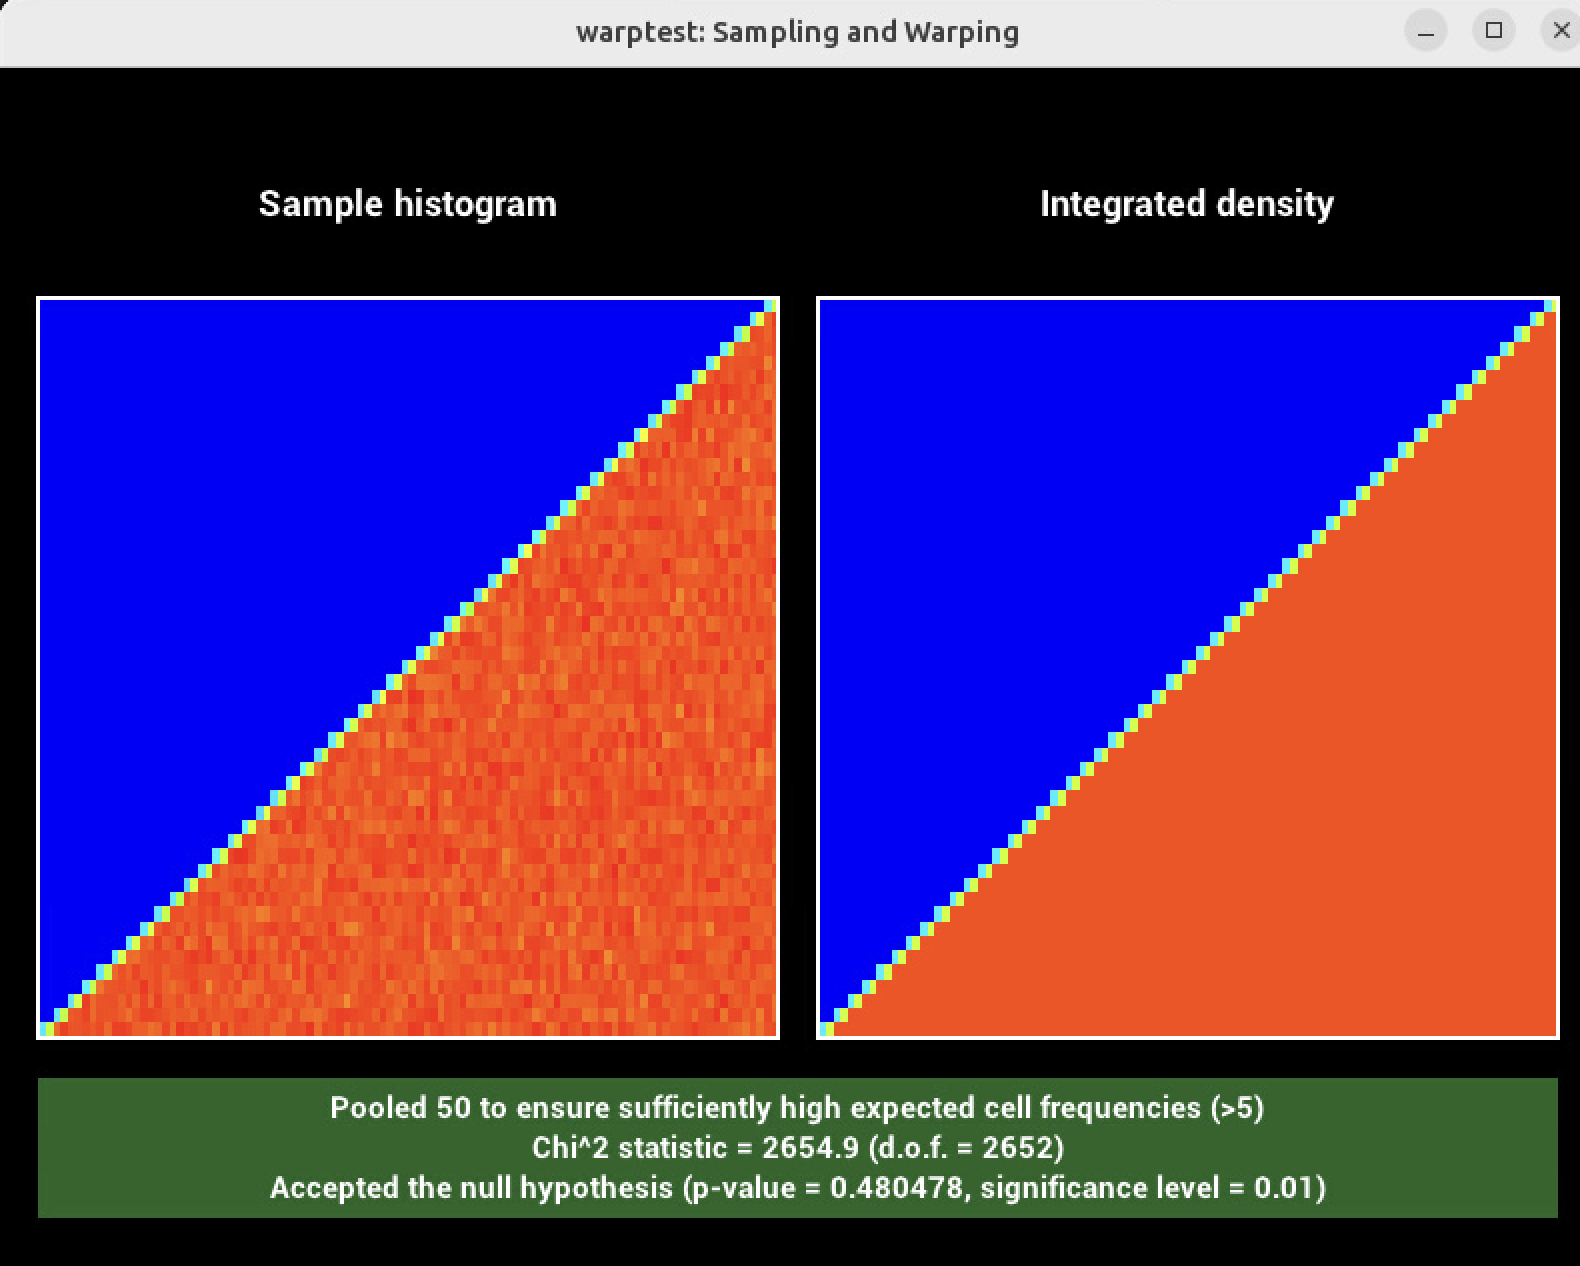
\includegraphics[width=0.8\textwidth]{pictures/wrap_test.png}
 \caption{Warp test results}
 \end{figure}


\paragraph{Problem (b)}

Our PDF is proportional to $f(x,y) = xy$. However, because a PDF should integrate to 1, we need to normalize it:
\[
p(x,y) = \frac{f(x,y)}{\int_0^1 \int_0^1 f(x,y)\,dy\,dx}.
\]

We compute the normalization constant:
\[
\int_0^1 \int_0^1 xy\,dy\,dx = \frac{1}{4},
\]
which gives
\[
p(x,y) = 4xy.
\]

The joint CDF is
\[
F(x_o,y_o)
= \int_0^{x_o} \int_0^{y_o} 4xy\,dy\,dx
= x_o^2 y_o^2.
\]

We compute the marginal CDF of $x$:
\[
F_x(x_o) = F(x_o,1) = x_o^2.
\]

Applying the inverse CDF:
\[
x_i = F_x^{-1}(u) = \sqrt{u}.
\]

Next, we compute the conditional CDF:
\[
F_{y|x}(y_o \mid x_i)
= \frac{F(x_i,y_o)}{F(x_i,1)}
= y_o^2.
\]

Applying the inverse conditional CDF:
\[
y_i = F_{y|x}^{-1}(v \mid x_i) = \sqrt{v}.
\]

Thus, the resulting transformation is
\[
\boxed{(x_i,y_i) = (\sqrt{u},\,\sqrt{v})}.
\]
